\documentclass{report}
\usepackage[utf8]{inputenc}
\usepackage[english]{duomasterforside}
\usepackage{graphicx}
\usepackage{caption}
\usepackage{subcaption}

\begin{document}
\title{Master's Essay}
\duoforside[author={Adrian Eriksen}, dept={Department of Informatics}, program={Language Technology}]

\setcounter{secnumdepth}{0}

\section{Introduction}
In this essay I will explain the challenges of cross-domain sentiment analysis and how we might use transfer learning to solve it.
Sentiment analysis is the process of trying to understand the sentiment behind a statement or document using machine learning. This can, among other things, be used to get information from reviews that can provide useful information.
There are many different ways to formulate a sentiment. A movie review might state "The movie is not bad at all.". If we simply look for words like "bad" and classify them as negative, we will get inaccurate results.\\\\
First, I will explain some of the technologies that has created the foundation for what we now use in language technology.
\\\\  - Structure of essay - \\\\
Pretraining:\\ 
BERT\\
ELMO\\
task specific\\

%Number sections

\newpage


\section{Sentiment Analysis}
Sentiment analysis (SA) is the computational treatment of opinions, sentiments and subjectivity of texts. SA is also known by opinion mining and a few other terms, and has a variety of different applications. It can be used for labelling reviews of movies or books, opinion mining from sites like Twitter and determining whether a written text is casual, informative or friendly, like Grammarly.\\\\
One of the original challenges with SA was that sentiment is rarely identifiable by keywords alone \cite{pang-etal-2002-thumbs}. When humans are presented with the task of selecting a set of key words to tell whether a movie review is positive or negative, our intuition often leads us towards words like "horrible", "boring" and "sucks" for negative reviews, and "excellent", "thrilling" and "amazing" for positive reviews. As it turns out, selecting words like these gives us a much lower accuracy than if we train a model on labelled reviews, letting the model figure out which words are important. One of the challenges that is raised by training on a specific domain (e.g movie reviews), is that it transfers poorly to other domains like restaurant reviews. In the movie review domain, some of the words that carries negative weight is words like "2", "series" and "tv", which makes sense in that specific domain (people tend to disfavor movies based on tv series, and sequels), but this is obviously not applicable while trying to predict whether a review of a restaurant is positive or negative \cite{taboada-etal-2011-lexicon}.
%Mention different granularities word/sentence/intensities just mention variations
%Talk about lexicon vs other methods
%
%Discuss different datasets
%What has been done for SA in Norwegian?
%Domain effects for SA
%NoReC

\section{NoReC}
The Norwegian Review Corpus (NoReC) is a dataset containing more than 35,000 full-text reviews from Norwegian news sources \cite{11509/124}.\\
NoReC covers a range of different domains, including literature, movies, video games, restaurants, music and theater, in addition to product reviews across a range of categories. Each review is labelled with a score ranging from 1-6, provided by the author of the review. NoReC was primarily created for training and evaluating models for document-level sentiment analysis, which makes it ideal for testing differences between domains on a document-level.
%Get more specific numbers
%Transition into domain adaptation
%Set up tables with counts etc

\begin{figure}[h!]
	\begin{subfigure}{.33\textwidth}
	\centering
	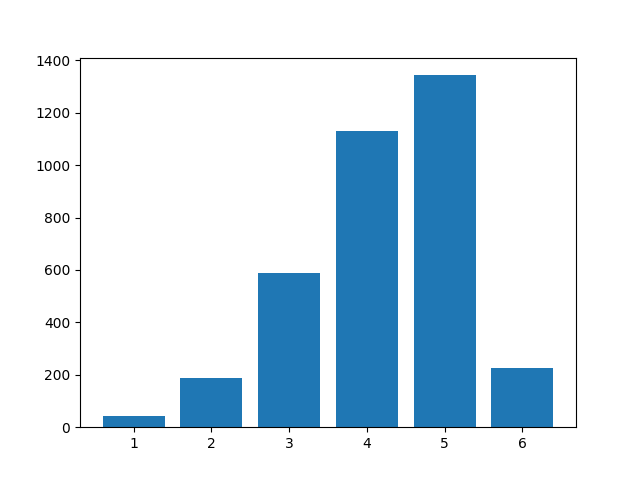
\includegraphics[width=1\linewidth]{img/dev_ratings}
	\caption{development}
	\label{fig:devratings}
	\end{subfigure}%
	\begin{subfigure}{.33\textwidth}	
	\centering
	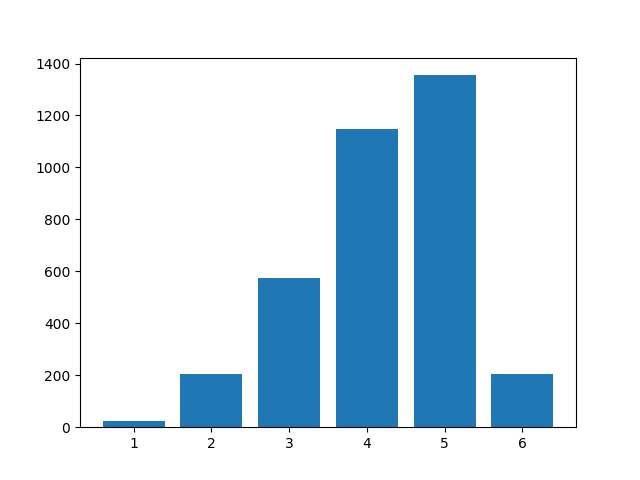
\includegraphics[width=1\linewidth]{img/test_ratings}
	\caption{test}
	\label{fig:testratings}
	\end{subfigure}%
	\begin{subfigure}{.33\textwidth}
	\centering
	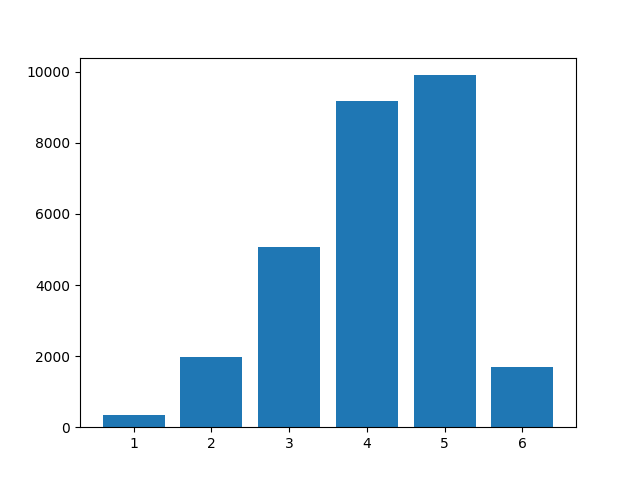
\includegraphics[width=1\linewidth]{img/train_ratings}
	\caption{training}
	\label{fig:trainratings}
	\end{subfigure}
\end{figure}

\begin{figure}[h!]
	\begin{subfigure}{.33\textwidth}
		\centering
		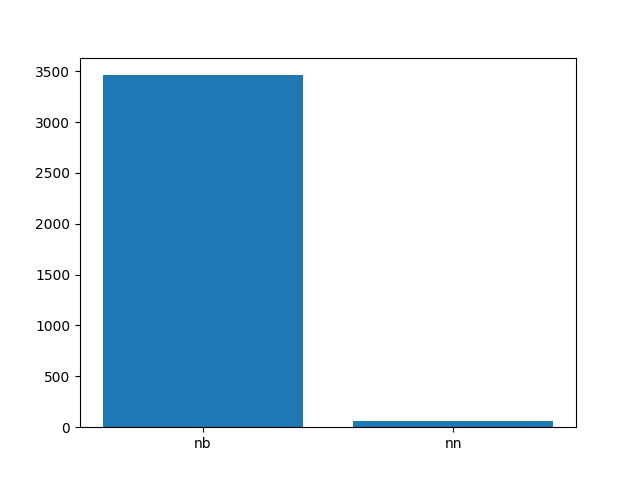
\includegraphics[width=1\linewidth]{img/dev_lngs}
		\caption{development}
		\label{fig:devlngs}
	\end{subfigure}%
	\begin{subfigure}{.33\textwidth}	
		\centering
		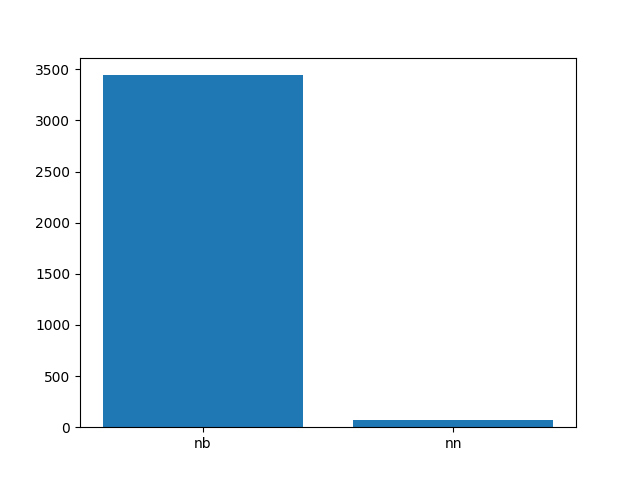
\includegraphics[width=1\linewidth]{img/test_lngs}
		\caption{test}
		\label{fig:testlngs}
	\end{subfigure}%
	\begin{subfigure}{.33\textwidth}
		\centering
		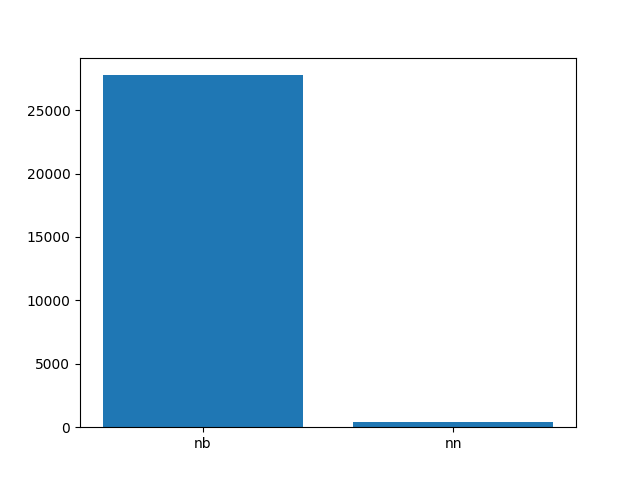
\includegraphics[width=1\linewidth]{img/train_lngs}
		\caption{training}
		\label{fig:trainlngs}
	\end{subfigure}
\end{figure}

\noindent
\section{Transfer Learning}
Transfer learning is a means to exract knowledge from a source setting and apply it to a different target setting. For example, one could train a model to recognize dogs, and then apply the knowledge to a model trying to recognize wolves. In NLP this can be especially useful, because words often means the same in a given context. There are, however, a few different types of transfer learning. One is when you have labeled data in the source domain and adapt the knowledge to different domains, also known as domain adaptation. A different, more common approach, is training on a large amount of unlabeled data, before adapting the representations using self supervised learning.

%\section{Preprocessing}
%Pretraining languange models is one of the key components of natural language processing. Historically we have pretrained a model for a single task. If we wanted to make a model that can predict whether a movie review is positive or negative, we would feed the model a large amount of labelled reviews so that it may learn the differences. The challenges this raises lies in how exactly this data should be stored in the model, and figuring out what to focus on when learning. In NLP there are a lot of ways to approach text processing. The most intuitive way might be to split the words by sentences (punctuations) and whitespaces (words) and have the model learn which words and sentences are the most recurring in the different reviews, disregarding universally common words like 'the'. In addition, n-grams have been used to try and get a deeper understanding of context. Instead of only looking at one word at a time, we look at the current word as well as the n previous words. This is just one of many techniques that can be applied to improve the model. Others include POS-tagging, NP chunking and Named Entity Recognition to mention some.\\\\
%\noindent
%There are however a couple of challenges when considering the different types of text processing for pretraining language models. A lot of text processing requires a large amount of manual labour beforehand. While splitting sentences and words in most cases are a trivial task for a program to solve, POS-tagging and NER are not. There is a fairly large amount of data that already have this, namely the Brown Corpus, but limiting language models to only learn from one source would be crippling in regards to making newer and better models. In addition, if we would feed all the additional information about every word and sentence to the model, the computational power required would be insurmountable.

\section{Pretraining}
\noindent
The large amount of information that each word could contain, turned out to be solvable by vectorization (embedding). It was discovered that by mapping each word to a vector, we could keep a lot of it's properties without having to process all of it's information. By looking at which words appeared in the same context, we could place synonyms close to eachother in the vector space. If we take the example of the words "king" and "queen", they would be placed close to eachother in the vector space, along with words like "royalty" and "palace". However, "queen" would be closer to "female", while "king" would be closer to "male". One of the main problems remained, however. Training the embeddings on a large dataset is still very expensive in both time, energy and resources.
\noindent
\subsection{Vectorization}
ELMo - Embeddings from Language Models was the next step in the evolution of word vectorization \cite{Peters:2018}. Where we previously assigned a vector to each word, ELMo looks at the context the word appears in. If we take the word "fall", this could have multiple meanings. One being the verb "to fall", another being the time of year as in "autumn". With traditional embeddings, we would learn the vectors based on a dataset and assign only one vector to "fall". One of the revolutionary things that ELMo did, is that each token is assigned a representation that is a function of the entire input sentence. In other words, the embedding assigned to "fall" is calculated from the sentence it appears in. The way ELMo does this, is by using a bidirectional long short-term memory (BiLSTM) RNN to calculate the probability of both previous and future words in the sentence, before returning the contextualized embedding.

\subsection{Finetuning}
BERT - Bidirectional Encoder Representations from Transformers is probably the most influential invention in NLP in recent years \cite{DBLP:journals/corr/abs-1810-04805}. Upon it's release in 2018, it obtained state-of-the-art results on eleven NLP tasks in a variety of fields. Whereas previous language representation models like OpenAI GPT had been unidirectional, BERT uses attention mechanisms to learn the contextual relations between words. The way BERT does this is by using a "masked language model" (MLM) pre-training objective. First, the model replaces some of the words in the dataset with the [MASK] token, then the model attempts to predict the actual value of the token, based on the context provided by the unmasked words in the sentence. Next, the model does "next sentence prediction" (NSP). By pairing 50\% of the sentences in the dataset, BERT is tasked with predicting whether the next sentence in a document is actually the next sentence, with a 50\% chance it will be. This has proven very useful for tasks like question answering, where models are required to produce fine-grained output at the token level. Upon the release of the paper Google also released the models used in the paper, BERT$_{BASE}$ and BERT$_{LARGE}$. These are both increadibly large models with 110M and 340M parameters respectively. Training a model of this size requires an enormous amount of computational power, energy and time. By making both the code and pre-trained models from the paper publicly available, it became possible for small research groups with limited computational power and funding, to fine-tune BERT and apply it as they saw fit.
%Pretraining word representations has become (one of the key components) of neural language understanding models in recent years. The main goal of pretraining word representations is to model complex characteristics of word use and how these uses vary across linguistic contexts.~\cite{https://www.aclweb.org/anthology/N18-1202.pdf}
%When we pretrain word representations, we usually do so on a large text corpus. 
\section{Domain Adaptation}
Domain Adaptation is the part of transfer learning where you want to apply the model trained during the pretraining to a target domain.
\subsection{Domain Adaptation for Sentiment Analysis}

%After all this: Talk about specific papers that deals with the problems I've discussed.


\newpage
\bibliography{refs}
\bibliographystyle{apalike}
\end{document}